
\section{Technical Lemmas for Chapter \ref{ch:kinetic}} \label{sec:appendix}
%\appendix

We prove here the averaging lemma used throughout this chapter.  
This lemma is an immediate corollary of \cite{Be} Theorem 6.  It is merely a localization of that result.  
\begin{lemma}[Averaging Lemma]\label{thm:avg_lemma}
Let $\Omega$ be an open subset of space-time $\R \times \R^n$, and $\bar{\Omega}$ a compact subset of $\Omega$.  

For any smooth function $\eta \in \Ctest(\R^n)$ and any $m \in \R^+$, there exists a constant $C = C(n,m,\eta, \bar{\Omega}, \Omega)$ and a constant
\[ \alpha = \frac{1}{2(1+m)} \]
such that the following is true:

For any two functions $f$ and $g$ in $L^2(\Omega \times \R^n)$ satisfying
\[ \kinet f = g, \]
it is true that
\[ \norm{\int \eta f \,dv}_{H^\alpha(\bar{\Omega})} \leq C \paren{\norm{f}_{L^2(\Omega \times \R^n)} + \norm{\bessel^{-m/2} g}_{L^2(\Omega\times\R^n)}}. \]
%
%Assume that
%\[ \kinet f = g. \]
%Then for any smooth function $\eta \in \Ctest(\R^n)$ and any $m \in \R^+$, there exists a constant $C = C(n,m,\eta, \bar{\Omega}, \Omega)$ and a constant
%\[ \alpha = \frac{1}{2(1+m)} \]
%such that
%\[ \norm{\int \eta f \,dv}_{H^\alpha(\bar{\Omega})} \leq C \paren{\norm{f}_{L^2(\Omega \times \R^n)} + \norm{\bessel^{-m/2} g}_{L^2(\Omega\times\R^n)}}. \]
\end{lemma}

By $\norm{g}_{H^\alpha(\bar{\Omega})}$, we mean the infimum of $\norm{\tilde{g}}_{H^\alpha(\R^{n+1})}$ over all extensions $\tilde{g}$ of $g$ to $\R^{n+1}$.  

\begin{proof}
Let $\phi(t,x)$ be a smooth function supported on $\Omega$ and identically equal to 1 on $\bar{\Omega}$.  Then
\[ \kinet (\phi f) = \phi g + f \kinet \phi. \]
By \cite{Be} Theorem 6,
\[ \norm{\phi \int \eta f \,dv}_{H^\alpha(\R \times \R^n)} \leq C \paren{\norm{\phi f}_{L^2(\R \times \R^n \times \R^n)} + \norm{\bessel^{-m/2} \paren{\phi g + f \kinet \phi}}_{L^2(\R \times \R^n \times \R^n)}}. \]
Because $\bessel^{-m/2}$ is a bounded operator from $L^2$ to $L^2$, and because $\phi$ is a smooth function supported on $\Omega$ and depending only on $t$ and $x$, 
\[ \norm{\bessel^{\frac{-m}{2}} \paren{\phi g + f \kinet \phi}}_{L^2(\R^{1+2n})} \leq C(\phi) \norm{\bessel^{\frac{-m}{2}}g}_{L^2(\Omega\times \R^n)} + C(m,\phi)\! \norm{f}_{L^2(\Omega\times\R^n)}\!. \]

The result follows.  
\end{proof}

The following is a technical lemma about the geometry of cones.  We use it at the very end of the proof of Proposition~\ref{thm:DG2.kinetic}.  

\begin{figure}[h]
\centering
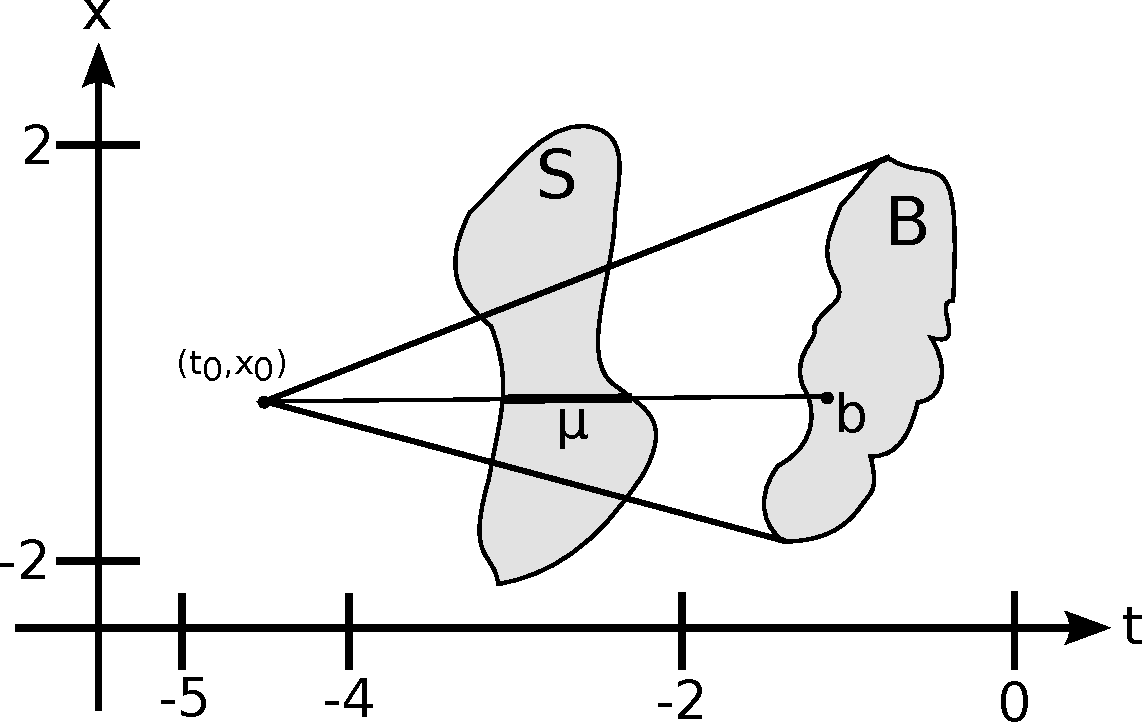
\includegraphics[width=.5 \textwidth]{NFP-diagram-Cone}
\caption{A diagram showing the assumptions of Lemma~\ref{thm:cone}.}
\end{figure}

\begin{lemma}\label{thm:cone}
Let $\mathcal{C} \subseteq \R \times \R^n$ be a cone from a vertex $(t_0,x_0) \in [-5, -4] \times B_2$ to a base set $B \subseteq [-2,0]\times B_2$.  % having $(t_0,x_0) \in [-5, -4] \times B_2$ and $B \subseteq [-2,0]\times B_2$.  
Let $S$ be a subset of $\R\times\R^n$ such that for each $b \in B$, the line segment connecting $(t_0,x_0)$ to $b$ intersects $S$ on a set with Hausdorff $\mathcal{H}^1$ measure at least $\mu$.  

Then 
\[ \abs{\mathcal{C} \cap S} \geq \frac{ |B| \mu^2}{80}. \]
\end{lemma}

\begin{proof}
Let $A(t)$ be the cross-sectional area of our cone at time slice $t$.  If $\mathcal{H}^n$ is the Hausdorff measure of dimension $n$, we write
\[ A(t) = \mathcal{H}^n\paren{\mathcal{C} \cap \bracket{\{t\}\times \R^n}}. \]
By the nature of cones, $A(t_0)=0$, $A$ is affine for $t_0 < t < -2$, then sub-affine for $-2<t<0$, and $A(t)=0$ for $t > 0$.  Specifically,
\[ A(t) = \frac{A(-2)}{-2-t_0} \paren{t-t_0} \qquad t_0 < t < -2, \]
\[ A(t) \leq \frac{A(-2)}{-2-t_0} \paren{t-t_0} \qquad -2 \leq t. \]


Since $B$ is contained in $\mathcal{C} \cap [-2,0]\times \R^n$, 
\[ |B| \leq \int_{-2}^0 A(t) \,dt \leq \int_{-2}^0 \frac{A(-2)}{-2-t_0}\paren{t-t_0} \,dt = \frac{A(-2)}{-2-t_0} \bracket{t_0^2 - (2+t_0)^2}/2 \leq 4 A(-2). \]

This means that 
\[ A(-2) \geq \frac{|B|}{4}. \]

Now we have a lower bound on the size of the cone, so for $t_0 \leq t \leq -2$
\begin{equation}\label{lower_bound_on_A} 
A(t) \geq \frac{|B|}{4(-2-t_0)}(t - t_0). 
\end{equation}

%Since $A(t)$ is increasing in $t$, the total measure of $\mathcal{C}\cap S$ will be smallest when $S$ is located near the vertex.  Each segment intersects $S$ on a set with measure at least $\mu$, and a segment of length $\mu$ can fit inside the cylinder $[t_0,t_0+x]\times B_2$ $\mu^2 = 4^2 + x^2$, $x = \sqrt{\mu^2 - 16}$.  At its most slant, a segment goes up $-2-t_0$ and over $4$, so with an extent $t$ you get rise $t$ and run $4t/(-2-t_0)$ for a length$^2$ of $t^2 + 16t^2/(2+t_0)^2$ or $t^2 \paren{1 + 16/2^2} = 5t^2$.  
%
%Consider a point $b \in B$ and the line segment from $(t_0,x_0)$ to $b$, which intersects $S$ on a set of measure at least $\mu$.  Because $A(t)$ is increasing in $t$, this intersection contributes more 

Consider the map from $B$ to $\{0\}\times\R^n$ given by stereographic projection from the point $(t_0,x_0)$, and let $db$ be a probability measure on $B$ proportional to the pullback of $\mathcal{H}^n \rest_{\{0\}\times\R^n}$ under this projection.  %In other words, $db(E)$ is the probabilty that a ray from $(t_0,x_0)$ to $B$ will intersect $E$.  
%Let $db$ be a probability measure on $B \subseteq \R \times \R^n$ which is a pullback of the stereographic projection, with pole $(t_0,x_0)$, from $\R \times \R^n$ to a copy of $\R^n$.  It measures what percentage of the rays from $(t_0,x_0)$ intersect a region of $B$.  
Then $db$ represents the proportion of any time-slice of $\mathcal{C}$ generated by rays through a given portion of $B$.  

To find the measure of $\mathcal{C} \cap S$, we must ask how much each time slice intersects $S$, or in integral form
\[ \abs{\mathcal{C} \cap S} = \int_{t_0}^{0} A(t) \int_{b \in B} \indic{(t,x) \in \mathcal{C} \cap S} \,dbdt. \]
By Fubini, this becomes
\begin{equation}\label{measure_of_intersection} 
\abs{\mathcal{C} \cap S} = \int_{b \in B} \int_{t_0}^0 A(t) \indic{(t,x) \in \mathcal{C} \cap S} \,dtdb. 
\end{equation}

From the definition of $\mu$ and the arc length formula,
\[ \mu \leq \int_{t_0}^0 \indic{(t,x) \in \mathcal{C} \cap S} \sqrt{1 + |b-x_0|^2/(-2-t_0)^2} \,dt \leq \sqrt{5} \int_{t_0}^0 \indic{(t,x) \in \mathcal{C} \cap S}. \]

Because $A(t)$ is increasing and $\indic{(t,x) \in \mathcal{C} \cap S}$ integrates to at least $\mu/\sqrt{5}$, 
\[ \int_{t_0}^0 A(t) \indic{(t,x) \in \mathcal{C} \cap S} \,dt \geq \int_{t_0}^{t+\mu/\sqrt{5}} A(t) \,dt. \]
From this bound, \eqref{measure_of_intersection}, and \eqref{lower_bound_on_A} we can at last compute
\[ \abs{\mathcal{C} \cap S} \geq \frac{|B|}{4(-2-t_0)} \int_{t_0}^{t_0 + \mu/\sqrt{5}} (t-t_0) \,dt = \frac{|B|}{4(-2-t_0)} \frac{\mu^2}{10} \geq \frac{|B|\mu^2}{80}. \]
\end{proof}

The following lemma is a commonly known fact about mollifiers.  Despite being known, a proof is surprisingly difficult to find in the existing literature.  Therefore, in the interest of completeness, we prove it here.   

\begin{lemma}\label{thm:convolution_estimate}
Let $\eta\in \Ctest(\R^n)$ be such that the sequence $\eta_\eps(v) = \eps^{-n} \eta(v/\eps)$ is an approximation to the identity.  There exists a constant $C=C(n,s,\eta)$ such that, for any $g \in H^s(\R^n)$, 
\[ \norm{g - g\ast \eta_\eps}_{L^2(\R^n)} \leq C \norm{g}_{H^s(\R^n)} \eps^s. \]
\end{lemma}

\begin{proof}
The bound is easy to compute by taking the Fourier transform and using Plancharel's theorem:
\begin{align*} 
\norm{g - g\ast \eta_\eps}_{L^2}^2 &= \int \hat{g}^2 \paren{1 - \hat{\eta_\eps}}^2 \,d\xi 
\\ &\leq \int (1+\xi^2)^s \hat{g}^2 \,d\xi \,\, \sup_{\xi} \frac{\abs{1-\hat{\eta_\eps}(\xi)}^2}{(1+\xi^2)^s}
\\ &= \norm{g}_{H^s(\R^n)}^2 \,\, \sup_{\xi} \frac{\abs{1-\hat{\eta_\eps}(\xi)}^2}{(1+\xi^2)^s}.
\end{align*}

Since $\eta \in \Ctest$, the fourier transform $\hat{\eta}$ is Lipschitz with some constant $\bar{C}$. Thus $\hat{\eta_\eps}(\xi) = \hat{\eta}(\eps \xi)$ is Lipschitz with constant $\bar{C}\eps$.  Since $\eta_\eps$ is an approximation to the identity, $\hat{\eta_\eps}(0) = 1$ and $\abs{\hat{\eta_\eps}(\xi)} \leq 1$ for all $\xi$.  Thus
\[ \abs{1 - \hat{\eta_\eps}(\xi)} \leq \min(2,\bar{C}\eps|\xi|). \]
%
%Our goal is to bound
%\begin{align*} 
%\norm{g - g\ast \eta_\eps}_{L^2}^2 &= \int \hat{g}^2 \paren{1 - \hat{\eta_\eps}}^2 \,d\xi 
%\\ &\leq \int (1+\xi^2)^s \hat{g}^2 \frac{\min(2,C\eps|\xi|)^2}{(1+\xi^2)^s} \,d\xi. 
%\end{align*}

The function $\frac{\min(2,\bar{C}\eps\xi)^2}{(1+\xi^2)^s}$ achieves its maxumum value at the critical point $\bar{C}\eps|\xi| = 2$, and that maximum value is 
\[ \frac{2^2}{\paren{1+\paren{\frac{2}{\bar{C}\eps}}^2}^s} = \frac{4 \eps^{2s}}{\paren{\eps^2 + 4/\bar{C}^2}^s} \leq C \eps^{2s}. \]
\end{proof}


%-----------------------------------------------------------------------------
%-----------------------------------------------------------------------------
%-----------------------------------------------------------------------------


\section{Technical Lemmas for Chapter \ref{ch:SQG}} \label{sec:technical}

In this appendix we state and prove a few technical lemmas.  

\begin{lemma}[De Giorgi Iteration Argument] \label{thm:DG1 skeleton}
For any constant $\bar{C} \geq 0$, there exists a $\delta>0$ such that the following holds:

Let $\Omega \subseteq \R^2$ be a bounded open set with $C^{2,\beta}$ boundary for some $\beta \in (0,1)$.  
Let $f \in L^2([-2,0]\times\Omega)$ be a function with the property that for any positive constant $a$
\begin{equation} \label{DG energy ddt} \ddt \int (f-a)_+^2 + \int \abs{\Lambda^{1/2} (f-a)_+}^2 \leq \bar{C} \paren{ \int \indic{f \geq a} + \int (f-a)_+ + \int (f-a)_+^2 }. \end{equation}

Then
\[ \int_{-2}^0 \int (f-0)_+^2 \,dxdt \leq \delta \]
implies that
\[ f(t,x) \leq 1 \qquad \forall t\in[-1,0], x \in \Omega. \]
\end{lemma}

\begin{proof}
Consider for $k \in \N$ the constants $t_k := -1 - 2^{-k}$ (so that $t_0 = -2$ and $t_\infty = -1$), and functions
\[ f_k := (f - 1 + 2^{-k})_+ \]
(so that $f_0 = (f)_+$ and $f_\infty = (f-1)_+$).  

Define
\[ \E_k := \int_{t_k}^0 \int_\Omega f_k^2 \,dxdt. \]

When $f_{k+1}>0$, then in particular $f_k \geq 2^{-k-1}$.  Thus for any finite $p$, there exists a constant $C$ so
\begin{equation} \label{non-linearization} \indic{f_{k+1}>0} \leq C^k f_k^p. \end{equation}
\vskip.3cm

Let $k\geq 0$ and define $\eta:[-2,0] \to \R$ a continuous function
\[ \eta(t) := \begin{cases}
0 & t \leq t_k \\
2^{k+1} (t-t_k) & t_k \leq t \leq t_{k+1} \\
1 & t_{k+1} \leq t.
\end{cases} \]

Let $s \in (t_{k+1},0)$.  Multiplying the inequality \eqref{DG energy ddt} with cutoff $a_k$ by $\eta(t)$ and integrating in time from $-2$ to $s$, then integrating by parts, we obtain
\[ \int f_k(s,x)^2\,dx - 2^{k+1} \int\displaylimits_{t_k}^{t_{k+1}} \int f_k(t,x)^2 \,dxdt + \int\displaylimits_{t_{k+1}}^s \HDint{1/2}{f_k} \,dxdt \leq \bar{C} \paren{ \int\displaylimits_{t_k}^0 \int \indic{f_k>0} + f_k + f_k^2 \,dxdt } \]
By taking the supremum over all $s \in (t_{k+1},0)$, we obtain
\begin{equation} \label{DG energy sup}
\sup_{[t_{k+1},0]} \int f_k^2 \,dx + \int_{t_{k+1}}^0 \HDint{1/2}{f_k}\,dxdt \leq C \paren{ 2^{k+1} \int_{t_k}^0 \int f_k^2\,dxdt + \int_{t_k}^0 \int \indic{f_k > 0} + f_k \,dxdt } 
\end{equation}
\vskip.3cm

From Proposition~\ref{thm:hadamard 3 lines} and Sobolev embedding, 
\[ \int_{t_{k+1}}^0 \paren{ \int f_k^4 \,dx }^{1/2} \,dt \leq C \int_{t_{k+1}}^0 \HDint{1/2}{f_k} \,dxdt. \]
Therefore by the Riesz-Thorin interpolation theorem,
\[ \int_{t_{k+1}}^0 \int f_k^3 \,dxdt \leq C \paren{ \sup_{[t_{k+1},0]} \int f_k^2 \,dx + \int_{t_{k+1}}^0 \HDint{1/2}{f_k} }^{3/2}. \]
This estimate, along with \eqref{DG energy sup} and \eqref{non-linearization}, and the fact that $t_{k-1} < t_k$ and $f_{k-1} \geq f_k$, tell us that
\[ \int_{t_{k+1}}^0 \int f_k^3 \,dxdt \leq C^k \E_{k-1}^{3/2}. \]

Now we can estimate, using again \eqref{non-linearization} and the fact $f_k \geq f_{k+1}$,
\[ \E_{k+1} \leq C^k \int_{t_{k+1}}^0 \int f_k^3 \,dxdt \leq C^k \E_{k-1}^{3/2}. \]
\vskip.3cm

This nonlinear recursive inequality $\E_{k+1} \leq C^k \E_{k-1}^{3/2}$, by a standard fact about nonlinear recursions (see \cite{DG} or \cite{Va.dg}), tells us that there exists a constant $\delta$ depending only on $C$ (which in turn depends only on the constant $\bar{C}$ in \eqref{DG energy ddt})
\[ \E_0 \leq \delta \textrm{ implies } \lim_{k \to \infty} \E_k = 0. \]

By assumption
\[ \E_0 = \int_{-2}^0 \int (f)_+ \leq \delta. \]
Therefore $\E_k \to 0$ and, by the dominated convergence theorem,
\[ \int_{-1}^0 \int (f-1)_+ \,dxdt = 0. \]

The result follows.  
\end{proof}

%\label{thm:Holder interpolation}

\begin{lemma} \label{thm:interpolation C1 to holder}
Let $\alpha \in (0,1)$.  There exists a constant $C = C(\alpha)$ such that, for any set $\Omega$ and any $f \in C^{0,1}(\Omega)$,
\[ \bracket{f}_\alpha \leq C \norm{f}_\infty^{1-\alpha} \norm{\grad f}_\infty^\alpha. \]
\end{lemma}

\begin{proof}
This simple lemma is a straightforward calculation:
\begin{align*} 
\sup_{x,y \in \Omega} \frac{|f(x)-f(y)|}{|x-y|^\alpha} &= \sup |f(x)-f(y)|^{1-\alpha} \paren{\frac{|f(x)-f(y)|}{|x-y|}}^\alpha 
\\ &\leq \paren{2 \norm{f}_\infty}^{1-\alpha} \paren{ \sup \frac{|f(x)-f(y)|}{|x-y|} }^\alpha
\\ &\leq C \norm{f}_\infty^{1-\alpha} \norm{\grad f}_\infty^\alpha.
\end{align*}
\end{proof}

\begin{lemma} \label{thm:interpolation holder to C1}
Let $\alpha \in (0,1)$ and $\Omega$ a set that satisfies the cone condition.  There exist constants $C = C(\alpha, \Omega)$ and $\ell = \ell(\Omega)$ such that, for any $f \in C^{1,\alpha}(\Omega)$
\[ \norm{\grad f}_\infty \leq C \paren{ \delta\n \norm{f}_\infty  + \delta^\alpha \bracket{\grad f}_\alpha }\]
for all $\delta < \ell$.  
\end{lemma}

The idea of the proof is to average $\grad f$ along an interval of length $\delta$ with endpoint $x$.  The magnitude of the average will be small, since $f \in L^\infty$, and the average will differ not very much from $\grad f(x)$ since $\grad f \in C^{1,\alpha}$.  

\begin{proof}
Since $\Omega$ satisfies the cone condition, there exist positive constants $\ell$ and $a<1$ such that, at each point $x \in \bar{\Omega}$, there exist two unit vectors $e_1$ and $e_2$ such that $|e_1\cdot e_2| \leq a$ and $x + \tau e_i \in \Omega$ for $i=1,2$ and $0 < \tau \leq \ell$.  In other words, $\Omega$ contains rays at each point that extend for length $\ell$, end at $x$, and are non-parallel with angle at least $\cos\n(a)$.  

Consider the directional derivative $\del_i f$ of $f$ along the direction $e_i$, and observe that for any $0 < \delta \leq \ell$,
\begin{equation} \label{average bounded by Linfty} \abs{\int_0^\delta \del_i f(x + \tau e_i) \,d\tau} = \abs{f(x+\delta e_i) - f(x)} \leq 2 \norm{f}_\infty. \end{equation}

On the other hand, $\del_i f$ is continous so, for any $\tau \in (0,\ell]$,
\[ \abs{\del_i f(x) - \del_i f(x+\tau e_i)} \leq \bracket{\grad f}_\alpha \tau^\alpha. \]
From this, we obtain that
\[ \int_0^\delta \del_i f(x + \tau e_i) \,d\tau \leq \int_0^\delta \paren{\del_i f(x) + \bracket{\grad f}_\alpha \tau^\alpha } \,d\tau = \delta \del_i f(x) + \bracket{\grad f}_\alpha \frac{\delta^{1+\alpha}}{1+\alpha} \]
and a similar bound holds from below.  Thus
\[ \abs{ \delta \del_i f(x) - \int_0^\delta \del_i f(x + \tau e_i) \,d\tau} \leq \bracket{\grad f}_\alpha \frac{\delta^{1+\alpha}}{1+\alpha}. \]

Combining this bound with \eqref{average bounded by Linfty}, we obtain
\[ \abs{\del_i f(x)} \leq \frac{2}{\delta} \norm{f}_\infty + \frac{\delta^\alpha}{1+\alpha} \bracket{\grad f}_\alpha. \]

This bound is independent of $x$ and of $i=1,2$.  Since $e_1 \cdot e_2 \leq a$ by assumption, by a little linear algebra we can bound $\grad f$ in terms of the $\del_i f$ and obtain that, for all $\delta \in (0,\ell]$,
\[ \norm{\grad f}_\infty \leq \frac{C}{1-a^2} \paren{ \delta\n \norm{f}_\infty + \delta^\alpha \bracket{\grad f}_\alpha }. \]

\end{proof}



\begin{lemma} \label{thm:technical scaling of barrier}
There exist constants $\bar{\lambda} > 0$ and $\alpha > 1$ such that, for any $0 < \eps \leq 1/2$ and any $z \geq 1$
\[ \paren{|\eps\n (z - 1) + 3|^{1/4} - 2^{1/4}}_+ - \alpha \paren{|z|^{1/4} - 2^{1/4}}_+ \geq \bar{\lambda}. \]
\end{lemma}

\begin{proof}
For $z$ fixed, this function is increasing as $\eps$ decreases, so it will suffice to show the lemma when $\eps = 1/2$, that is to show
\[ f_\alpha(z) := \paren{|2 z + 1|^{1/4} - 2^{1/4}}_+ - \alpha \paren{|z|^{1/4} - 2^{1/4}}_+ \geq \bar{\lambda} \]
for all $z \geq 1$.  Note that $f_\alpha(z) \geq f_\beta(z)$ if $\alpha < \beta$.  

For $z \geq 2$, 
\[ f_\alpha(z) = (2z+1)^{1/4} - 2^{1/4} - \alpha z^{1/4} + \alpha 2^{1/4} = z^{1/4} \paren{(2 + 1/z)^{1/4} - \alpha} + (\alpha-1)2^{1/4}. \]
For any $\alpha < 2^{1/4}$, clearly $f_\alpha(z)$ tends to $\infty$ as $z$ increases. Therefore there exist $N$ and $\alpha_0 > 1$ such that 
\[ f_\alpha(z) \geq 1 \qquad \forall z \geq N, \alpha\leq \alpha_0. \]
\vskip.3cm

We can decompose $f_\alpha(z) = g_1(z) - (\alpha - 1) g_2(z)$ where
\begin{align*} 
g_1(z) &:= \paren{|2 z + 1|^{1/4} - 2^{1/4}}_+ - \paren{|z|^{1/4} - 2^{1/4}}_+, \\
g_2(z) &:= \paren{|z|^{1/4} - 2^{1/4}}_+. 
\end{align*}
Note that $g_1$, $g_2$ are both continuous, and $g_1(z)$ is strictly positive for $z \geq 1$.  Therefore we can take $\alpha \in (1,\alpha_0]$ small enough that
\[ \alpha - 1 < \frac{\inf_{[1,N]} g_1}{\sup_{[1,N]} g_2}. \]

For this $\alpha$, $f_\alpha(z)$ is strictly positive on the compact interval $[1,N]$, and $f_\alpha(z) \geq 1$ on $[N,\infty)$.  Therefore $f_\alpha(z)$ has a positive lower bound $\bar{\lambda}$ for all $z \geq 1$.  
\end{proof}